\documentclass[11pt]{article}
% Supplementary Material for "The Wrong Unit of Uncertainty".
% Secondary material relocated from the main manuscript, content-unchanged.
\usepackage[T1]{fontenc}
\usepackage[margin=1in]{geometry}
\usepackage{amsmath,amssymb,amsthm}
\usepackage{graphicx}
\usepackage{booktabs}
\usepackage{natbib}
\usepackage[ruled,vlined]{algorithm2e}
\usepackage{hyperref}
\usepackage{xcolor}

\newtheorem{theorem}{Theorem}
\newtheorem{proposition}{Proposition}
\newtheorem{lemma}{Lemma}
\newtheorem{corollary}{Corollary}
\theoremstyle{definition}
\newtheorem{assumption}{Assumption}
\newtheorem{definition}{Definition}
\theoremstyle{remark}
\newtheorem{remark}{Remark}

\graphicspath{{figures/}}
\newcommand{\Ftilde}{\widetilde{F}}
\newcommand{\rhohat}{\widehat{\rho}}
\DeclareMathOperator{\SE}{SE}

% Number figures/tables/sections with an "S" prefix for the online supplement.
\renewcommand{\thefigure}{S\arabic{figure}}
\renewcommand{\thetable}{S\arabic{table}}
\renewcommand{\thesection}{S\arabic{section}}

\title{Supplementary Material for\\
``The Wrong Unit of Uncertainty:\\
Adaptive Design-Aware Conformal Inference for\\
Repeated Cross-National Surveys''}
\author{The Authors}
\date{}

\begin{document}
\maketitle

This online supplement collects secondary material referenced from the main
manuscript. All content, numbers, and figures are reproduced unchanged; only figure
numbers carry an ``S'' prefix.

\section{The finite-$K$ mechanism and the development grid}\label{sup:mechanism}

\paragraph{Development: why the third gate is needed.} On a Gaussian grid with known
truth ($K\in\{30,60,120,240\}$, $\rho$ up to $1.8$), the selector transitions from
PCB to deconvolution at $\rho_0$ and to conservative at large $\rho$; but a naive
deconvolution that omits gate~B \emph{undercovers} at small $K$---coverage falls to
$0.75$ at $K=30$ in the transition zone---because the target scale is estimated from
few countries (Figure~\ref{fig:selector}). Adding the finite-$K$-safe scale lifts
this to $0.82$, and the reliability gate B lifts the deployed worst cell to
$0.862$ while abstaining to conservative wherever the remainder cannot be bounded.
These four transition cells at $0.862$--$0.878$ are the development evidence that
\emph{motivates} the safety gate and \emph{calibrates} $\widehat\delta_{\text{UCB}}$;
they are not reused below.

\paragraph{The finite-$K$ mechanism, isolated.} A controlled Gaussian illustration
(design SD $=$ transport SD, $\rho{=}0.9$; \texttt{fig\_theory\_illustration.py})
makes the source of the undercoverage explicit and shows why the deployed rule is a
selector rather than a deconvolver. Both the naive and the finite-$K$-safe
deconvolved score scales lie \emph{below} the oracle $s_R/s_{\text{plug}}$ at small
$K$ (Figure~\ref{fig:shrinkage}): subtracting a design-noise variance estimated from
few countries over-shrinks the scale, and the resulting band is too narrow. The safe
guard shrinks less, and both converge to the oracle as $K\to\infty$. The coverage
consequence is severe and grows with the trajectory length $L$ that the band must
hold simultaneously (Figure~\ref{fig:coverage_LK}): naive deconvolution falls to
$0.43$ at $K{=}25,\,L{=}16$, and the finite-$K$-safe scale improves it but does not by
itself reach nominal at small $K$. The deployed adaptive selector detects that the
remainder cannot be bounded and abstains to the conservative branch, remaining valid
throughout at a width cost---the mechanism behind the $K{=}320$-only activation in
the confirmatory holdout in the main text.

\begin{figure}[t]\centering
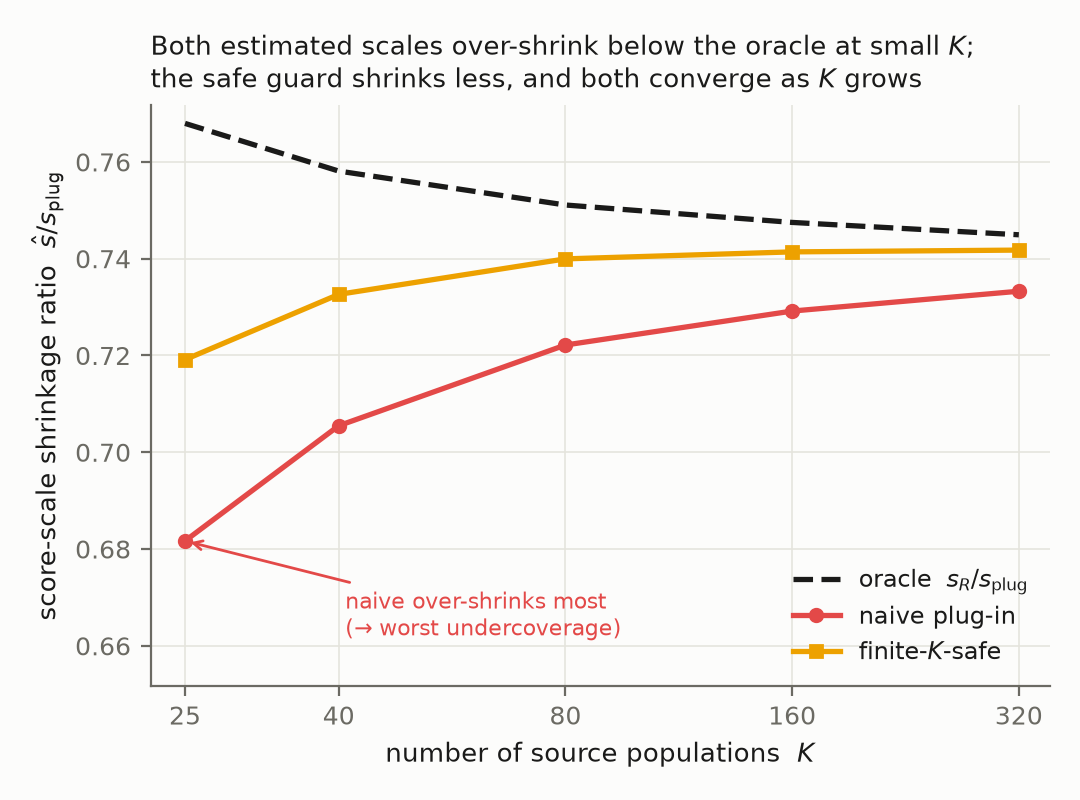
\includegraphics[width=.62\textwidth]{theory_shrinkage.png}
\caption{Score-scale shrinkage ratio $\hat s/s_{\text{plug}}$ vs $K$ (Gaussian
illustration, $\rho{=}0.9$, $L{=}8$). Naive and finite-$K$-safe deconvolution both
over-shrink below the oracle at small $K$---the source of the finite-$K$
undercoverage---with the safe guard shrinking less; both converge as $K$
grows.}\label{fig:shrinkage}
\end{figure}

\begin{figure}[t]\centering
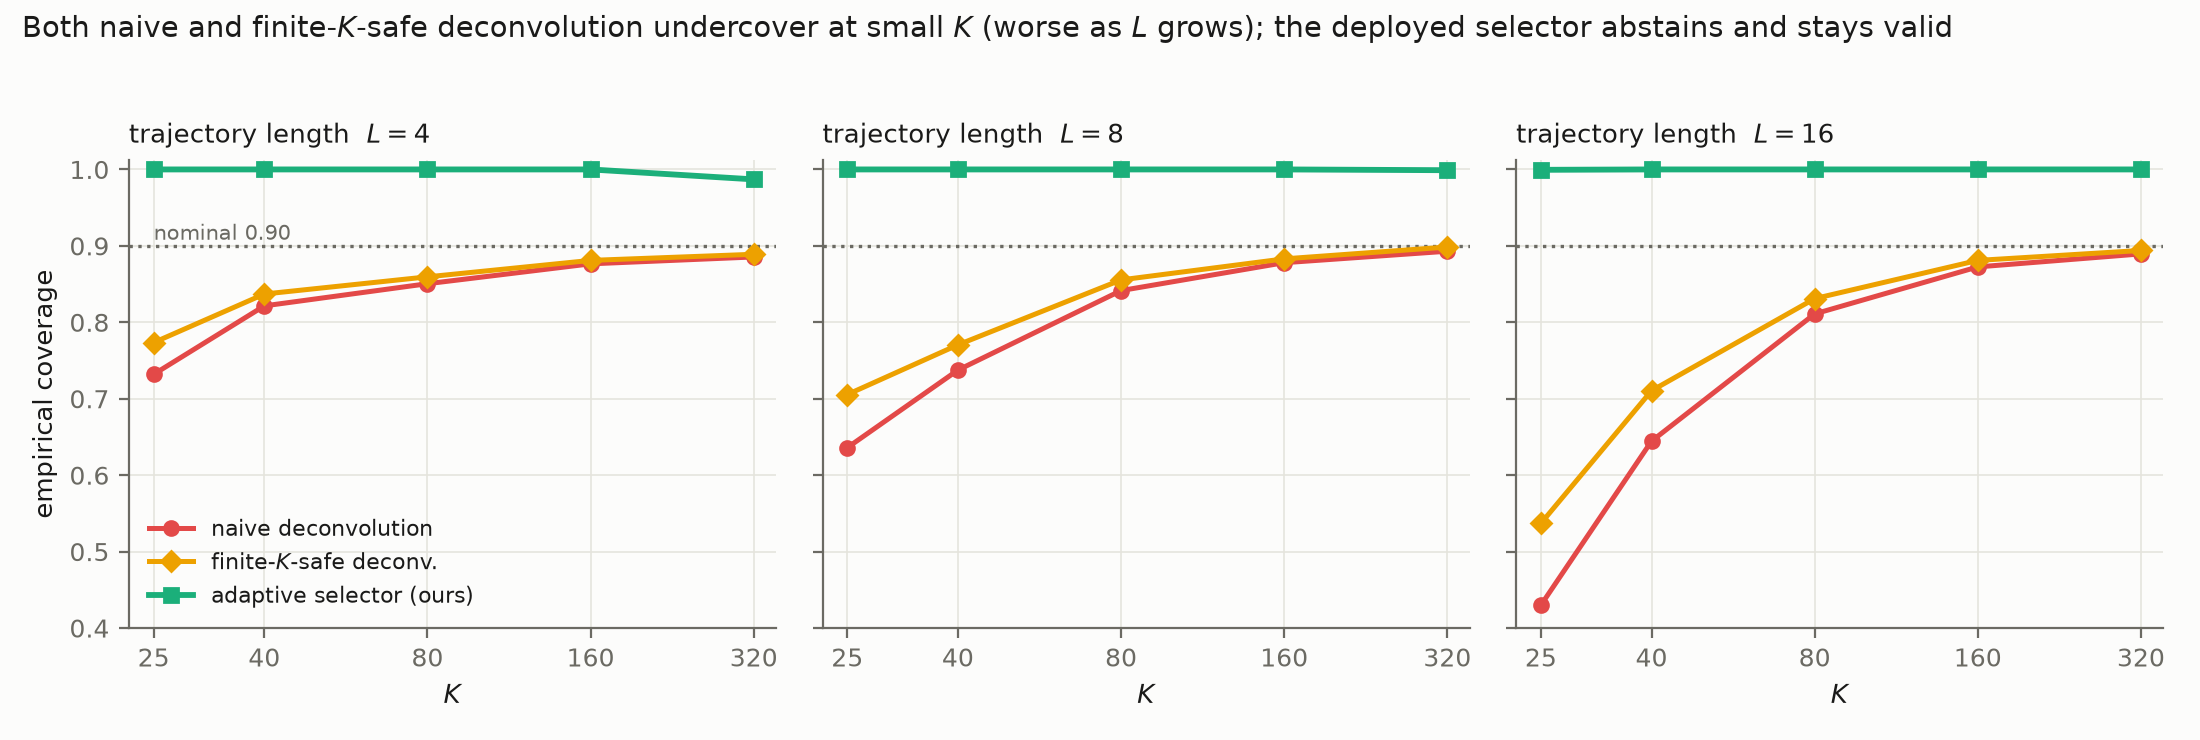
\includegraphics[width=\textwidth]{theory_coverage.png}
\caption{Latent-target coverage of the deconvolution branches vs $K$, faceted by
trajectory length $L$ (Gaussian illustration, $\rho{=}0.9$; nominal $0.90$ dotted).
Naive deconvolution undercovers severely at small $K$ and worse as $L$ grows; the
finite-$K$-safe scale improves but does not itself reach nominal at small $K$. The
deployed adaptive selector abstains to conservative and stays valid
throughout.}\label{fig:coverage_LK}
\end{figure}

\begin{figure}[t]\centering
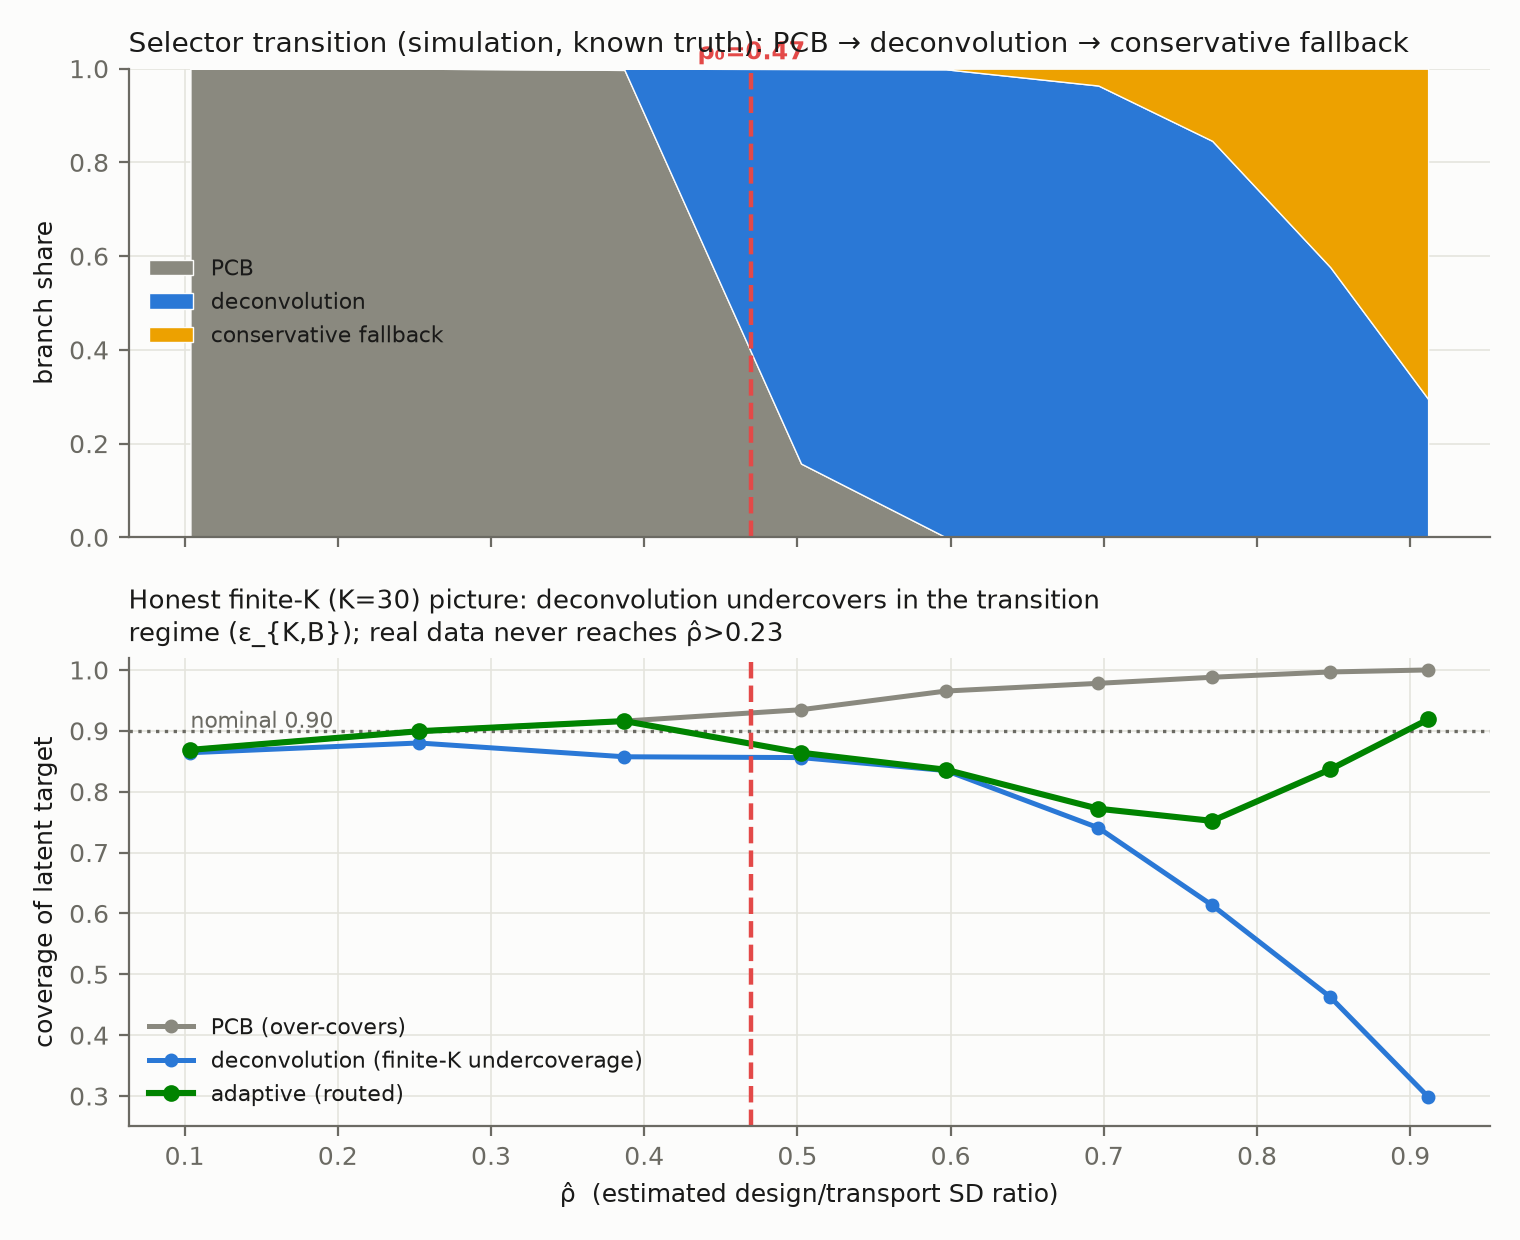
\includegraphics[width=.78\textwidth]{selector_sweep.png}
\caption{Development grid (Gaussian, known truth). The selector transitions
PCB\,$\to$\,deconvolution\,$\to$\,conservative as $\rho$ grows; naive deconvolution
undercovers at small $K$ in the transition zone---the finite-$K$ remainder the safety
gate controls.}\label{fig:selector}
\end{figure}

\section{Extended robustness of the remainder bound}\label{sup:robustness}

\paragraph{Cell-by-cell resolution of the base-method deficit.} On the holdout the
studentized band's worst deployed cell was $0.843$ (weak cross-round dependence at
$K{=}25$), a finite-$K$ self-inclusion deficit worst at small $K$ and long trajectories.
After switching to the unstudentized clustered band, a preregistered rerun on a fresh
grid ($K\in\{15,\dots,60\}$, ten DGPs) confirms the fix: the worst cell rises from
$0.802$ (S2, $K{=}15$) to $0.893$, every cell meets its exact floor, and the width cost
is $1.02$--$1.05\times$ on the real ESS transport bands (trust-CDF errors are
$\approx$homoskedastic across the low-trust core, so the constant-width band is
competitive; the only cells where it pays more than $10\%$ are synthetic heavy-tailed
curves at $K{=}15$, where the studentized alternative is itself invalid).

\paragraph{Extreme-tail behavior of the remainder bound.} Beyond the base-method deficit
resolved by deploying the unstudentized clustered band, the holdout exposed a second,
extreme-tail limitation. The Gaussian-calibrated
remainder bound $\widehat\delta_{\text{UCB}}$ is not robust at the extreme: in $77$ of
$360{,}000$ draws ($0.02\%$), on strongly-dependent or heavy-tailed DGPs at $K{=}320$ and
$\rho\ge0.72$, draws that pass gate~B undercover to $\approx0.79$; because the gates route
$96$--$98\%$ of draws in those cells to conservative, the deployed cell coverage there is
nonetheless $0.95$--$0.996$.

\section{Additional empirical robustness}\label{sup:empirical}

\paragraph{Design-preserving stress test.} Subsampling the real AmericasBarometer
while preserving its stratified-PSU structure, the estimated $\rho$ \emph{saturates}
near $0.23$: since $s_{\text{plug}}^2=s_R^2+\overline{v^2}$, shrinking the sample
inflates design noise and observed spread in lockstep. The deconvolution regime is
therefore unreachable even semi-synthetically at survey scale---direct evidence for the
regime characterization of the main text.

\paragraph{The barriers are not survey artifacts.} Both gates are distribution-free, so
the boundary should transfer to any conformal procedure calibrated on estimated objects
(the general remark of the main text). A simulation confirms it outside the survey
setting (\texttt{e29\_beyond\_surveys}): across Gaussian, heavy-tailed, skewed, and a
non-survey model-based small-area (MRP-style) calibration, the reliability floor
$D\ge\sqrt{2/(K-1)}$ holds in every case (minimum $D/\text{floor}\ge1.06$), and the gate
opens only at $K\approx130$--$150$---if anything a stronger barrier than the
floor-implied $K\ge94$. The one substantive difference is instructive: when a small
area's posterior noise is comparable to the between-area signal
($\rhohat_{\mathrm{LCB}}=0.54$ at a noise-to-signal ratio of $0.5$), the \emph{need} gate
does fire, unlike any cross-national survey. A many-area MRP application with appreciable
posterior uncertainty is therefore the setting where the deconvolution could actually
activate---the positive-result frontier the survey-scale impossibility leaves open.

\paragraph{The AmericasBarometer supplies the design effect the ESS lacks.} The ESS
releases design weights but limited cluster identifiers; the AmericasBarometer
releases full stratified-PSU structure, letting us compute a proper design
bootstrap. The design effect is real: the ratio of the proper stratified-PSU
standard deviation to a naive independent-resampling one has median
$\approx1.13$--$1.20$ and reaches $1.9$ in the most clustered country-years. The
proper band captures clustering variance the naive bootstrap misses. Yet
certification is coarse-robust: the design effect moves band \emph{width} but rarely
flips the binary decline decision, because the decision is dominated by the
between-country transport spread, not the within-country design noise---the same
low-$\rho$ fact, seen from the certification side.

\paragraph{Robustness across age groups (ESS).} A preregistered age-group analysis
(preregistered in \texttt{docs/YOUTH\_PREREGISTRATION.md}) reruns the same
certification within fixed age bands, changing nothing else. The ``only Greece''
result is not an artifact of pooling ages: it holds within the older (50+) group for
both outcomes and within the middle (30--49) group for trust in parliament, so the
persistent decline is concentrated in the older and middle adult population rather
than created by averaging. Youth (18--29) certify \emph{zero} persistent declines,
but we read this as an underpowered null rather than youth stability: only $17$ of
$30$ countries clear the preregistered minimum-sample gate for a single youth band,
and the smaller, noisier youth cells yield wider design-aware bands that certify
less---the small-$K$ scope condition of the simulation appearing on real
data. The analysis thus supports the headline while adding an honest caveat, and it
is emphatically \emph{not} a story of youth-led democratic disaffection.

\paragraph{Youth deconsolidation on the World Values Survey.} The youth claim in the
Foa--Mounk reanalysis is only half-supported: the young show \emph{more} persistent
decline in rating democracy essential ($7$ vs.\ $3$ countries) but \emph{not} in
openness to strongman or army rule ($0$--$1$ vs.\ $4$), against the ``youth embrace
authoritarianism'' reading.

\bibliographystyle{apalike}
\bibliography{refs}

\end{document}
